\chapter{Results}\label{chap:results}

Once everything had been put together, tests were done to conclude whether the system met the requirements of the researchers.

The setup was as follows: the tracking system was loaded with the Raspberry Pi camera and two GoPro Hero Sessions, one of which was set to record. Another GoPro was placed on a block next to the system, and set to wide angle mode - this acted as a control when comparison was necessary. Since the tests were oriented towards video footage, it is advised to watch a few sample recordings online to get a feel for how the system operates. {\color{red} embed link to saved footage!}

Due to time constraints, the tests performed were done on humans in a laboratory.

\section{Testing whether the system can track an object}
What follows is a series of tests which demonstrate the scenarios in which the tracker succeeds (or fails) to work.

\subsection{Aiming at a stationary object}
The first test demonstrated that the system can locate and rotate towards an object in a complex environment. While this initially resulted in the gimbal oscillating around the object, once the timing issues had been fixed, the system was able to smoothly aim at the object before stopping entirely.

The system was unphased by the movement of other objects in the frame, such as a pushed chair.


\subsection{Tracking a slow moving object}
Next, the system was made to track an object moving in a slow, straight line. The camera would track the object in a slightly jerky fashion for the first two seconds, before correctly estimating the objects velocity and tracking it smoothly. During steady state, the camera lagged behind a walking-pace object with an angle of approximately 10\textdegree, depending on the velocity of the object and the distance to the camera.

\begin{figure}[h!]
  \centering
  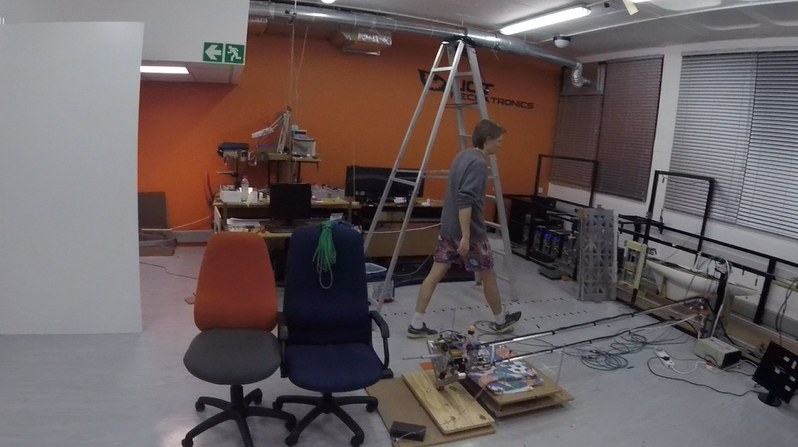
\includegraphics[width=\textwidth]{results/follow_walk_small_delay}
  \caption{\label{fig:follow_walk_small_delay}A photo of the system tracking a human walking at a slow pace.}
\end{figure}

\subsection{Tracking a fast moving object}
A test was done to see whether the system can track an object moving at higher velocities. It failed under either of two conditions:

If the object accelerated too quickly, the camera would sometimes fail to estimate the objects velocity before it left the frame and then rotate slowly towards the direction that the object had last been seen in.

If the object moved too quickly, the gimbal would fail to rotate fast enough and again lose sight of the object. However, if the object stopped or slowed down out of frame, the system would find it and start tracking properly again.


\subsection{Tracking a crouching or elevated object}
The system could adequately track an object at higher or lower pitch levels. Since more smoothing was applied to the Kalman Filter estimating the pitch of the object, the gimbal would take slightly longer to change its pitch accordingly.


\subsection{Tracking partially hidden objects}
Objects which were partially hidden (for example, a human behind a large chair or workspace divider) could still be adequately tracked. However, this stopped working when only the face of the tracked object was visible from 5 meters away.


\section{Testing the maximum angular tracking range}
Moving in a circle around the tracker empirically showed that the yaw rotation range was 175\textdegree, while the pitch could track from approximately -45\textdegree (before the system itself started obscuring the object) to 90\textdegree.

A GoPro Hero Session camera has a maximum field of view of 122\textdegree{} if set to the highest setting.

%\begin{figure}
%	\centering
%	\animategraphics[loop,autoplay,width=\textwidth]{12}{./tracking_cam_test_7/smaller_img}{0}{53}
%\end{figure}

\section{Testing the angular distortion effects}
To test and show the effects of distortion, two pictures taken in the same moment in time are shown below, in Figures~\ref{fig:distorted_gopro} and \ref{fig:less_distorted_gopro}.

\begin{figure}[h!]
  \centering
  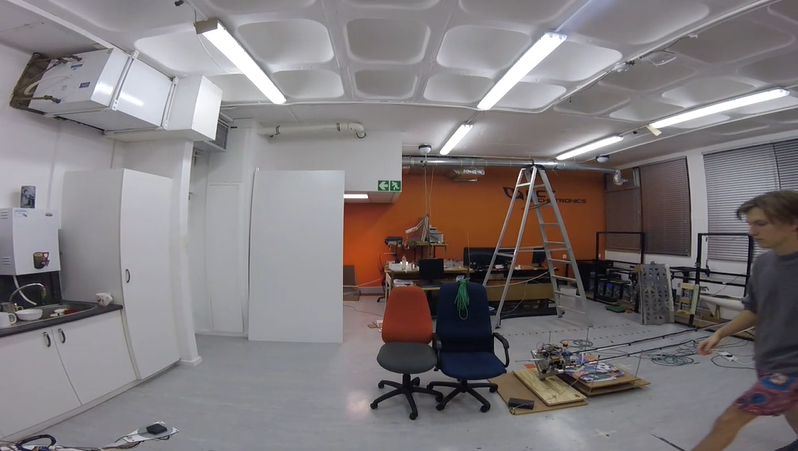
\includegraphics[width=\textwidth]{results/distorted_gopro}
  \caption{\label{fig:distorted_gopro}Photo from the stationary camera showing the distortions due to the cameras wide-angle mode.}
\end{figure}

\begin{figure}[h!]
  \centering
  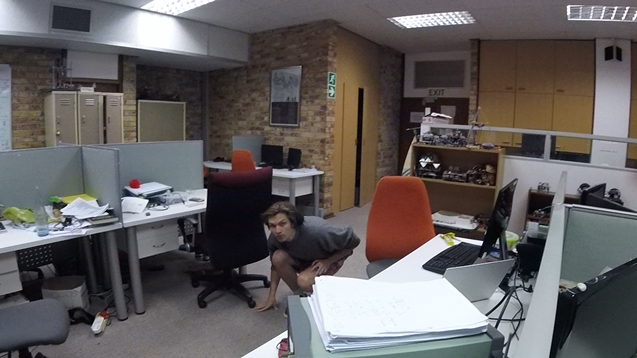
\includegraphics[width=\textwidth]{results/less_distorted_gopro}
  \caption{\label{fig:less_distorted_gopro}Photo from the rotating camera showing less distortion.}
\end{figure}

The distortion effects are easier to see when looking at straight lines (made to look curved) in the edges and corners of the image.




